%        File: HW01.tex
%     Created: 一 7月 09 06:00 下午 2018 C
% Last Change: 一 7月 09 06:00 下午 2018 C
%
\documentclass[UTF8,noindent]{ctexart}
\usepackage[a4paper,left=2.0cm,right=2.0cm,top=2.0cm,bottom=2.0cm]{geometry}
\usepackage{hyperref}
\usepackage{url}
\usepackage{graphicx}
\usepackage{amsmath}
\usepackage{amssymb}
\usepackage{enumitem}
\usepackage{tikz}
\usepackage{float}
\usepackage{listings}
\usepackage{xcolor}
\usepackage{forest}
\lstset{language = c,numbers=left, keywordstyle= \color{ blue!70 },commentstyle=\color{red!50!green!50!blue!50}, frame=shadowbox, rulesepcolor= \color{ red!20!green!20!blue!20 } 
} 
\usetikzlibrary{graphs}
\title{$Chapter\ 2-HW01$}
\author{$2015K8009929049$\ 冯吕}
\date{\today}
\begin{document}
\maketitle
\zihao{5}
\CJKfamily{zhsong}
$2.2.1$解:

$1)$生成串$aa+a*$的过程如下,以最左推导为例:
\[S\rightarrow S\ S\ * \rightarrow S\ S\ + \ S\ *\rightarrow a\ S\ +\ S\ *\rightarrow aa+\ S\ *\rightarrow aa+a*\]

$2)$该串的语法分析树如下:
\begin{figure}[H]
\centering
\begin{forest}
  [{$S$}
	[{$S$}
	  [{$S$}
		[{$a$}]
	  ]
	  [{$S$}
		[{$a$}]
	  ]
	  [{$+$}]
	]
	[{$S$}
	  [{$a$}]
	]
	[{$*$}]
  ];
\end{forest}
%\begin{tikzpicture}
%  \node {$S$}
%  child {node{$S$} child{node{$S$} child{node{$a$}}} child {node{$S$}child{node{$a$}}} child{node[left]{$+$}}}
%  child {node{$S$} child{node[right]{a}}}
%  child {node{$*$}};
%\end{tikzpicture}
\end{figure}

$3)$该文法生成的语言是运算数全为$a$,带有加法和乘法运算的后缀算术表达式的集合。

$4)$没有二义性。

$proof:$
\begin{itemize}
	\item 先证明一个该文法产生串的长度的结论:设串的推导过程中使用产生式$S\rightarrow S\ S\ +$和$S\rightarrow S\ S\ *$的次数为$m$,则串的长度为$L = 2\times m + 1$,且串中包含$m$个运算符和$m+1$个 a;
\begin{itemize}
  \item $1)$当$m=0$时,仅有$S\rightarrow a$一种情况,此时$L=1$,串由$1$个$a$和$0$个运算符构成,结论成立;
\item $2)$设当$m<k(k\ge 1)$时结论成立,则当$m=k$时,第一步推导必然为
\[S\rightarrow S_1S_2\ op\]
$op$为$+$或$*$。设$S_1\rightarrow \alpha, S_2\rightarrow \beta$, $\alpha, \beta$均为使用$S\rightarrow S_1S_2\ op$少于$k$次得到的串,设二者推导过程中分别使用该产生式$k_1$和$k_2$次,根据假设有:
\[L(\alpha) = 2*k_1 + 1, L(\beta) = 2*k_2+1\]
则串长度$L = L(\alpha) + L(\beta) + 1 = 2*(k_1+k_2+ 1) + 1= 2k+1$;且串中$a$的个数为$(k_1+1) + (k_2+1) = k+1$;运算符的个数为$k_1+k_2+1= k$,故结论成立。
\end{itemize}
\item 下面证明该文法无二义性,对串的长度做归纳。由前述证明可知,该文法产生的串长$L$可为任意非负奇数。对由该文法得到的长度为$K = 2*k+1$的串$w$:
  \begin{itemize}
	\item $1)$当$k=0$ 时,$L=1$,只有$S\rightarrow a$一种情况,显然没有二义性;
  \item $2)$设当$k<n$时结论成立。$S\rightarrow \omega$,根据$\omega$末尾运算符可确定第一步推导使用的产生式,不妨设为:
	\[S\rightarrow S_1S_2+\]
  从后向前处理串$\omega$,除去末尾的运算符,找到可以由$S$推导出的最短的串$\alpha$,设$\alpha$长度为$m_1$,由前述结论可知$m_1 = 2*k_1+1$,且$\alpha$包含$k_1$个运算符和$k_1+1$个$a$,由归纳假设可知$\alpha$无二义性,存在唯一的最左推导$S\rightarrow \alpha$;

  设串$\omega$剩余部分为$\beta$,设$\beta$的长度为$m_2$,同理可得$m_2 = 2*k_2+1$,$\beta$包含$k_2$个运算符与$k_2+1$个$a$,存在唯一最左推导$S\rightarrow \beta$,且满足$k = k_1+ k_2$。此时串$\omega$可表示成如下形式:
  \[\omega = \beta\alpha +\]

  故存在唯一的最左推导:
  \[S\rightarrow S\ S\ +\rightarrow \beta S\ + \rightarrow \beta \alpha +\]
  此时,仍不存在二义性。
  \end{itemize}
综上所述,该文法不具有二义性。
\end{itemize}


$2.2.5$解:

$1)proof:$\ 用归纳法证明:当生成的串的语法树的节点$\le 3$时,生成的串有$11, 1001$,对应的十进制的值为$3, 9$,能够被$3$整除。假设节点数$<n$的语法树生成的二进制串均能够被$3$整除,考虑节点数为$n$的语法树,它有下面两种可能的结构:
\begin{itemize}
  \item 情形一:
	\begin{figure}[H]
	  \centering
	  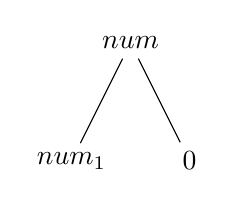
\begin{tikzpicture}
		\node{$num$}
		child{node{$num_1$} }
	  child{node{$0$}};
	  \end{tikzpicture}
	\end{figure}
  子树$num_1$的节点数$\le n$,因此,$num_1$生成的二进制串(记为$w_1$)能够被$3$整除,则$num$生成的二进制串(记为$w$):
  \[w=w_1 \times 2 \]
  也可以被$3$整除。
  \item 情形二:
	\begin{figure}[H]
	  \centering
	  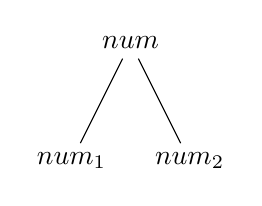
\begin{tikzpicture}
		\node{$num$}
		child{node{$num_1$}} 
		child{node{$num_2$}};
	  \end{tikzpicture}
	\end{figure}
	子树$num_1$和$num_2$的节点数均小于$n$,因此,它们生成的二进制串(分别记为$w_1$和$w_2$)能够被$3$整除,则$num$生成的二进制串(记为$w$):
	\[w = w_1\times 2^n + w_2\]
	也能够被$3$整除。
\end{itemize}
综上,该文法生成的二进制串能够被$3$整除。

$2)$不能。例如,对于二进制串$10101$,它的值为$21$,能够被$3$整除,但是不可以通过上面的文法推导出。\\

$2.3.1$解:制导翻译方案如下:
\begin{lstlisting}
E -> {print("+");} E1 + T
     |{print("-");} E1 - T
     |T

T -> {print("*");} T1 * F
     |{print("/");} T1 / F
     |F

F -> digit{print(digit)}
     |(expr)
\end{lstlisting}

表达式$9-5+2$对应的注释语法分析树如下:
\begin{figure}[H]
  \centering
  \begin{forest}
	[{$E.exp = +-952$}
	  [{$E.exp = -95$}
		[
		  {$E.exp = 9$}
		  [
			{$T.exp = 9$}
			[
			  {$F.exp = 9$}
			  [
				{$digit.expr = 9$}
			  ]
			]
		  ]
		]
		[
		  {$-$}
		]
		[
		  {$T.exp = 5$}
		  [
			{$F.exp = 5$}
			[
			  {$digit.expr = 5$}
			]
		  ]
		]
	  ]
	  [{$+$}]
	  [
		{$T.exp = 2$}
		[
		  {$F.exp  = 2$}
		  [
			{$digit.expr = 2$}
		  ]
		]
	  ]
	]
	%[
	%  {$expr$}, name = e
	%  [{$print("+")$},name = p1	]
    %  %
	%  [{$expr$}, name = e1
	%    [{$print("-")$}, name = p2]
	%    [{$expr$}, name=e3
	%      [{$term$}, name=e2
	%        [{$factor$}, name = f1
	%          [{$print("9")$}, name=p3]
	%          [{$9$}, name = c]
	%        ]
	%      ]
	%    ]
	%    [{$-$}, name = a1]
	%    [${term}$, name = t2
	%      [{$factor$}, name = f2
	%        [{$print("5")$}, name = p4]
	%        [{$5$}, name = c1]
	%      ]
	%    ]
	%  ]
    %  %
	%  [{$+$}, name = a2]
    %  %
	%  [{$term$}, name = t1
	%    [{$factor$}, name = f3
	%      [{$print("2")$}, name = p5]
	%      [{$2$}, name = c2]
	%    ]
	%  ]
	%];
  \end{forest}
\end{figure}
%输出结果为$+-952$.\\

表达式$9-5*2$对应的注释语法分析树如下:
\begin{figure}[H]
  \centering
  \begin{forest}
	[
	  {$E.exp = -9*52$}
	  [
		{$E.exp =9$}
		[
		  {$T.exp = 9$}
		  [
			{$F.exp = 9$}
			[
			  {$digit.expr = 9$}
			]
		  ]
		]
	  ]
	  [
		{$-$}
	  ]
	  [
		{$T.exp = *52$}
		[
		  {$T.exp = 5$}
		  [
			{$F.exp = 5$}
			[
			  {$digit.expr = 5$}
			]
		  ]
		]
		[
		  {$*$}
		]
		[
		  {$F.exp = 2$}
		  [
			{$digit.expr = 2$}
		  ]
		]
	  ]
	]
	%[{$expr$}
	%  [{$print("-")$}]
	%  [{$expr$}
	%    [{$term$}
	%        [{$factor$}
	%          [{$print("9")$}]
	%          [{$9$}]
	%        ]
	%    ]
	%  ]
	%  [{$-$}]
	%  [{$term$}
	%    [{$print("*")$}]
	%    [{$term$}
	%      [{$factor$}
	%        [{$print("5")$}]
	%        [{$5$}]
	%      ]
	%    ]
	%    [{$*$}]
	%    [{$factor$}
	%      [{$print("2")$}]
	%      [{$2$}]
	%    ]
	%  ]
	%]
  \end{forest}
\end{figure}
%输出结果为$-9*52$.


\end{document}


